\newpage
\section{Root functional modelling} \label{sec:functional}

Root growth is strongly influenced by pedo-climate conditions, and plant internal state. CPlantBox offers 'build in' ways to develop such models. 

CPlantBox is a bottom up model were root growth is first defined under perfect conditions. Adding mechanisms to take environmental conditions into account will alter the root system development by impeding root growth, and by changing soil allocation by roots due to root tropism and due to altered branching patterns.

In this section we assume static soil conditions, and demonstrate the predefined ways how the soil can affect root growth.
Dynamic soil conditions are described in the following section 'Model coupling'. 

Implemented root responses are the change in direction of the growing root tip, as described in Section \ref{sec:tropism}.
Further root response are 
\begin{itemize}
 \item scaling of the elongation rate 
 \item change of insertion angle
 \item change of lateral emergence probability
\end{itemize}

\subsection{Scaling the elongation rate} \label{sec:elongation}

Root elongation rate is influenced by water content, temperature, soil density, solutes, and many more. Regarding the processes that are investigated, various models can be applied. In CPlantBox the elongation rate is scaled with no predefined interpretation, i.e. we have to define a elongation rate scaling, which is dependent on such soil properties. The following example defines two compartments (one left, one right), where we change the scaling, and ca´n analyse the results. The same procedure will be used in Example \ref{sec:insertion_angle} and \ref{sec:branching}.

\lstinputlisting[firstline=1, language=Python, caption=Example 5a]{../../examples/python/example5a_elongation.py}

\begin{itemize}

\item[7-10] Creates the root system and opens the parameter file.

\item[13-17] We create a confining box with two overlapping boxes called left and right. These geometries are used for later analysis.

\item[20-24] We define a static soil properties using SDF (L23, L24) as we did in Section \ref{sec:hydro}. 
The left compartment has the value $minS$, the right $maxS$, between them is a linear gradient of length $slope$.

\item[27-31] Sets the scaling functions. L29 adjusts axial resolution and L30 tortuosity $sigma$. L31 sets the scale elongation function $f_{se}$ to the soil property. 

\item[34-39] Initialization and simulation loop. In a dynamic setting, $soilprop$ needs to be updated in each time step (comment L38).

\item[42-50] Analysis the root length in the left and right compartment. With parameters $minS$ and $slope$ only $21\%$ are located in the left compartment.

\item[53, 54] Writes the results for Paraview visualization (see Figure \ref{fig:elongation}).

\item[57] A vtk simulation of root lenghts. Press 'y' to obtain a x-z view of the root sytem to better see the effect. 

\end{itemize}

Next, we give a short layout, how the code would look like, if we take measured data (in this soil density versus depth), and include it in the simulation. 

\lstinputlisting[firstline=1, language=Python, caption=Example 5b]{../../examples/python/example5b_scaleelongation.py}

\begin{itemize}

\item[7-10] Creates the root system and opens the parameter file.

\item[12-18] In L12 an EquidistantGrid1D is created, which is a specialisation from SoilLookUp (in soil.hh). It represents a 1D grid as soil layers with scalar data attached to it. In L13, L14 we create example soil strength data. From this data we calculate the elongation scales (L15), and set it as grid data (L16). 

\item[L17, L18] Retrieve the elongation scale data at to points. The data is given per layer, no data interpolation is performed.

\item[20, 21] Sets the elongation scaling function to all root types.

\item[24-37] Simulation loop. If soil strength changes, the elongation scales must be calculated again (L32), and attached to the grid (L35).

\item[39,40] Exports results as vtp, and creates a vtk plot. The effect of the dense layer can not be seen in the results (between -10 and -20 cm depth, laterals will be shorter). An animation could reveal the effect. 

\end{itemize}

\begin{figure}
\begin{subfigure}[c]{0.3\textwidth}
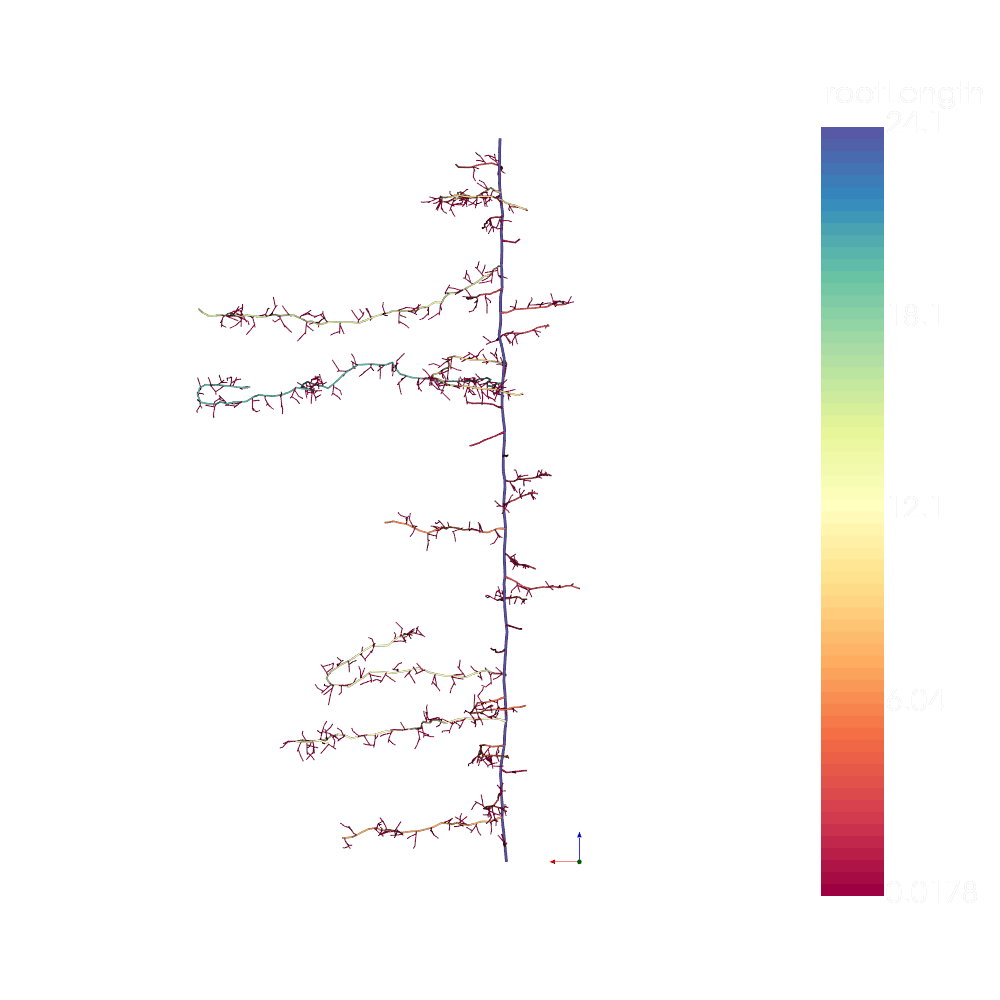
\includegraphics[width=0.99\textwidth]{example5a.png}
\subcaption{Root elongation rate} \label{fig:elongation}
\end{subfigure}
\begin{subfigure}[c]{0.3\textwidth}
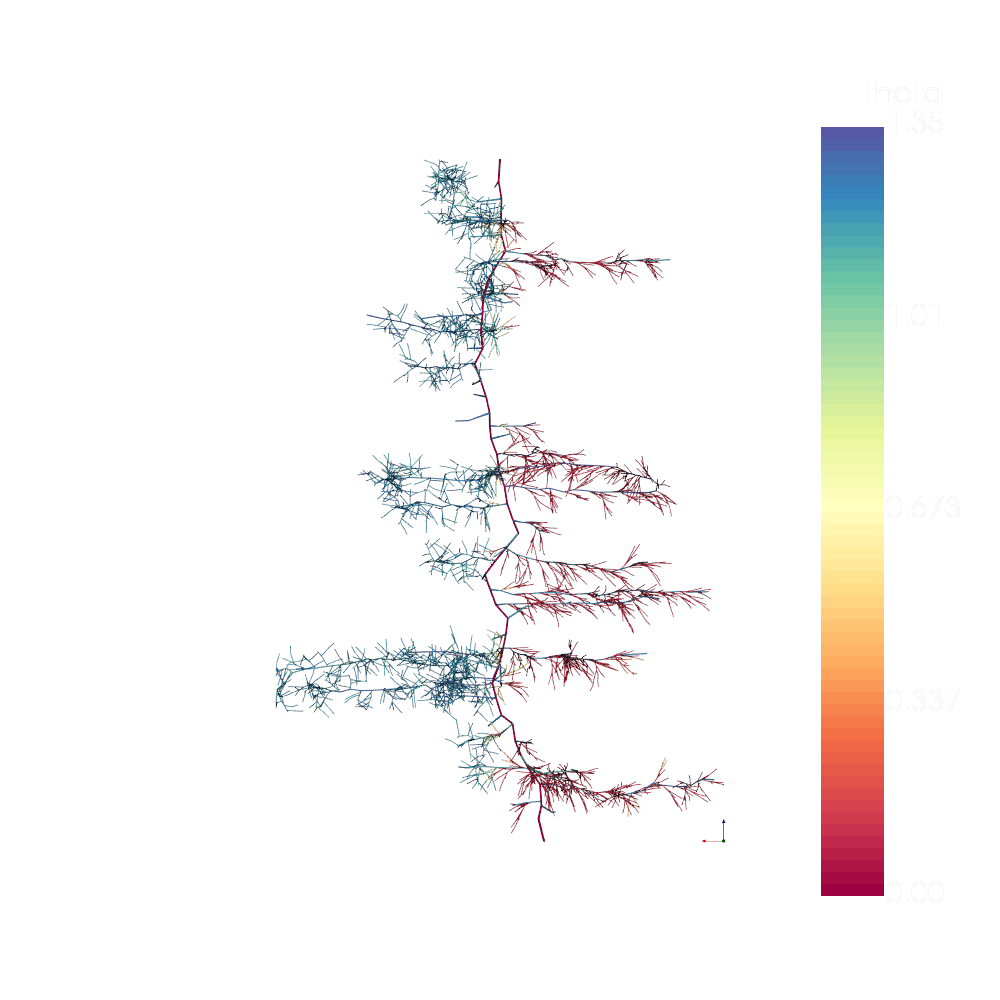
\includegraphics[width=0.99\textwidth]{example5c.png}
\subcaption{Insertion angle of laterals} \label{fig:insertion}
\end{subfigure}
\begin{subfigure}[c]{0.3\textwidth}
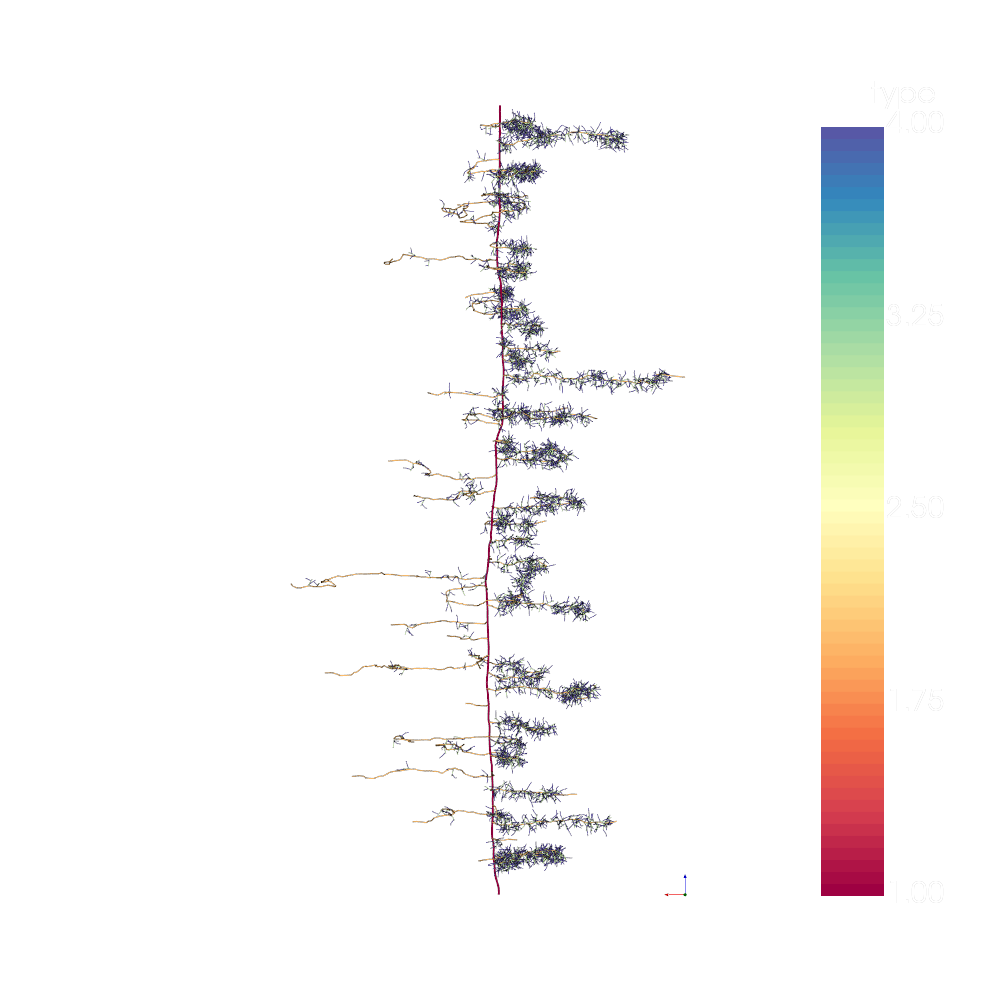
\includegraphics[width=0.99\textwidth]{example5d.png}
\subcaption{Branching density (probabilistic model)} \label{fig:probability}
\end{subfigure}
\caption{Predefined root responses (Example 5a)}
\end{figure}



\subsection{Change of insertion angle} \label{sec:insertion_angle}

The impact of nutrient concentration can influence the angle between parent roots and laterals (ref what else).

Analog to Example 5a two compartments are created, and the insertion angle is scale altered accordingly.

\lstinputlisting[firstline=1, language=Python, caption=Example 5c]{../../examples/python/example5c_insertionangle.py}

\begin{itemize}

\item[7-10] (as before) Creates the root system and opens the parameter file.

\item[13-17](as before) We create a confining box with two overlapping boxes called left and right. These geometries are used for later analysis.

\item[20-24] (as before) We define a static soil properties using SDF (L23, L24) as we did in Section \ref{sec:hydro}. 
The left compartment has the value $minS$, the right $maxS$, between them is a linear gradient of length $slope$.

\item[27-32] Sets the insertion angle scaling functions to second order laterals only (L29). L20 adjusts axial resolution and, L31 tortuosity $sigma$, and L32 sets the scale insertion angle function $f_{sa}$ to the soil property. Additionally, the maximal length of second order roots is redoubled. 

\item[34-39] Initialization and simulation loop.

\item[42-50] Analysis the root insertion angle in the left and right compartment. 

\item[53, 54] Writes the results for Paraview visualization (see Figure \ref{fig:insertion}).

\item[57] A vtk simulation of root lengths. Press 'y' to obtain a x-z view of the root system to better see the effect. 

\end{itemize}




\subsection{Cange of lateral emergence probability} \label{sec:branching}

Soil properies can affect branching patterns


\lstinputlisting[firstline=1, language=Python, caption=Example 5d]{../../examples/python/example5d_branching.py}

Note 0 never, systemic responses, getValue(x, organ) 


